\chapter{Aprendizaje estadístico}\label{Chapter1} 
% chktex-file 8
% chktex-file 12
% chktex-file 13
% chktex-file 44

Sea una cantidad cuantitativa $Y$, junto con $p$ predictores distintos, $X_1, X_2, \dots, X_p$. Se asume una relación entre $Y$ y $X = (X_1, X_2, \dots, X_p)$, que se puede escribir de forma general como 
\begin{equation}
Y = f(X) + \epsilon
\end{equation}  

\noindent donde $f$ es una función multivariable desconocida de los predictores y $\epsilon$ es un término de error aleatorio, independiente de $X$ y con media cero. En esta expresión, $f$ representa la información sistemática que proporciona $X$ acerca de $Y$. \\

En esencia, el aprendizaje estadístico hace referencia a una serie de métodos y aproximaciones para estimar $f$.

\section{Motivos para estimar $f$}

Algunos modelos pueden tener como objetivo la predicción y la inferencia. Por ejemplo, es el sector inmobiliario, se puede estar interesado en qué parámetros aumentan o disminuyen en mayor medida el precio de una propiedad o, conocer el valor de la misma a partir de sus características. Sin embargo, de forma general, estos problemas se tratan por separado. 

\subsection{Predicción}

En ocasiones, el conjunto de entradas $X$ está disponible fácilmente, mientras que para la salida $Y$ ocurre lo contrario. En este contexto, como el término de error tiene media cero, se puede predecir $Y$ a partir de 
\begin{equation}
\hat{Y} = \hat{f}(X)
\end{equation}

\noindent donde $\hat{f}$ representa la estimación de $f$ e $\hat{Y}$ representa la predicción para $Y$. Generalmente, se trata a la función $\hat{f}$ como una ``caja negra'', en el sentido de que no interesa la forma exacta, sino como de correctas son las predicciones. \\

El acierto de $\hat{Y}$ como predicción para $Y$ depende de dos cantidades: el error reducible y el irreducible. De forma general, $\hat{f}$ no será una estimación perfecta de $f$, y esta inexactitud introducirá cierto error. Este error es reducible porque, potencialmente, se puede mejorar la exactitud de $\hat{f}$ mediante el uso de técnicas de aprendizaje estadístico más adecuadas al problema. Sin embargo, incluso dando una estimación perfecta de $f$, es decir, $\hat{Y} = f(X)$, la predicción aún tendría error, ya que $Y$ también es función de $\epsilon$ que, por definición, es impredecible usando $X$. Por tanto, la variabilidad asociada a $\epsilon$ también afecta a la exactitud del modelo. Este es el conocido como error irreducible, ya que, por muy buena que sea la predicción de $f$; no se puede reducir. \\

Se puede demostrar que el error irreducible es mayor que cero. La cantidad $\epsilon$ puede contener variables que no se han medido y son útiles para predecir $Y$; al no medirlas, $f$ no las puede usar para predecir. Además, $\epsilon$ puede contener variaciones no mensurables; por ejemplo, el riesgo de una reacción adversa en un paciente puede variar dependiendo del día. \\

Sea una estimación $\hat{f}$ y un conjunto de predictores $X$ que conducen a una predicción $\hat{Y} = \hat{f}(X)$. Sean $\hat{f}$ y $X$ fijos entonces, se puede comprobar que 
\begin{equation}
E(Y - \hat{Y})^2 = E[ f(X) + \epsilon - \hat{f}(X)]^2 = \underbrace{[f(X) - \hat{f}(X)]^2}_{\text{reducible}} + \underbrace{\text{Var}(\epsilon)}_{\text{irreducible}}
\end{equation}

\noindent donde $E(Y - \hat{Y})^2$ representa la media, o valor esperado, de la diferencia al cuadrado entre el valor real y el predicho, y $\text{Var}(\epsilon)$ es la varianza asociada a al término de error $\epsilon$. \\

El error irreducible va a proporcionar siempre una cota superior (generalmente desconocida) en la exactitud de la predicción de $Y$.

\subsection{Inferencia}

En ocasiones, se tiene interés en conocer cómo afectan los cambios de los predictores $X_1, \dots, X_p$ al valor de $Y$. De este modo, el objetivo es estimar $f$ para conocer la relación entre $X$ e $Y$, es decir, cómo cambia $Y$ en función de cada uno de los predictores. Ahora el problema no es necesariamente hacer predicciones de $Y$, y $\hat{f}$ no puede ser tratada como una ``caja negra''. En este contexto, interesa contestar preguntas como las siguientes:
\begin{itemize}
\item ¿Qué predictores están asociados con la respuesta? Generalmente, solo una fracción pequeña de los predictores disponibles están asociados de forma sustancial con $Y$.
\item ¿Cuál es la relación de la respuesta con cada predictor?
\item ¿Se puede considerar la relación entre cada predictor e Y lineal, o es más compleja? Históricamente, muchos métodos para estimar $f$ consideran una forma lineal. En algunos casos, esto es razonable, pero en otros no basta para representar la relación entre las variables.
\end{itemize}

\section{Estimación de $f$}

Sea un conjunto de $n$ observaciones, denotadas como conjunto de entrenamiento (\textit{training data}), que se usarán para que el modelo aprenda a estimar $f$. Sea $x_{ij}$ el valor del predictor j-ésimo para la i-ésima observación. Entonces, el conuunto de entrenamiento tendrá la forma $\{(x_1, y_1), (x_2, y_2), \dots, (x_n, y_n)\}$, donde $x_i = (x_{i1}, x_{i2}, \dots, x_{ip})^T$. \\

Se busca encontrar una función $\hat{f}$ tal que $Y \approx \hat{f} (X)$ para una observación $(X, Y)$. De forma general, los métodos de aprendizaje estadístico se pueden distinguir en dos grupos: paramétricos y no paramétricos.

\subsection{Métodos paramétricos}

\noindent Estos métodos están basados en un modelo de dos fases:
\begin{itemize}
\item Primero, se asume la forma funcional de $f$. Por ejemplo, una hipótesis simple seria que $f$ es lineal en $X$
\begin{equation}
f(X) = \beta_0 + \beta_1 X_1 + \beta_2 X_2 + \dots + \beta_p X_p 
\end{equation}
Asumiendo que la relación es lineal, se reduce el problema de estimar una función p-dimensional arbitraria a la estimación de $p + 1$ coeficientes $\beta_\mu$, con $\mu = 0, 1, \dots, p$. 
\item Tras la elección del modelo, se necesita un proceso que use el conjunto de entrenamiento para ajustar o entrenar el modelo. En el caso del modelo lineal, se busca encontrar los valores de los parámetros $\beta_\mu$ tales que 
\begin{equation}
Y \approx \beta_0 + \beta_1 X_1 + \beta_2 X_2 + \dots + \beta_p X_p
\end{equation}
La aproximación más común para este caso es el método de mínimos cuadrados.
\end{itemize}

Esta aproximación en dos pasos se refiere como paramétrica, al reducir el problema de estimar $f$ a la estimación de un conjunto de coeficientes o parámetros. El problema de estos métodos es que la función elegida puede diferir en gran medida de la real, llevando a predicciones pobres. Se puede ser más flexible, ajustando a varias formas funcionales, pero esto puede conducir a un problema de \textit{overfitting}. 

\subsection{Métodos no paramétricos}

Estos métodos no hacen hipótesis explícitas sobre la forma funcional de $f$. Simplemente buscan una estimación de $f$ que se aproxime lo más posible a los datos del conjunto de entrenamiento, sin ser ni muy flexible ni muy rígido. Estos tienen la ventaja de que pueden encontrar una mayor variedad de formas de $f$. Sin embargo, al no reducir el problema de obtener $f$, necesitan un gran número de observaciones para obtener una buena estimación de $f$. 

\subsection{Exactitud vs interpretabilidad}

En inferencia, los modelos más retrictivos resultan mucho más interpretables que los flexibles, ya que dan una relación más clara entre cada predictor y la salida $Y$. En modelos de predicción, por el contrario, muchas veces no interesa la interpretabilidad sino la exactitud del resultado. En estos casos, se puede optar por modelos más flexibles (teniendo cuidado de no caer en problemas de \textit{overfitting}). De forma general, a mayor flexibilidad del modelo, menor interpretabilidad. 

\begin{figure}[h]
\centering
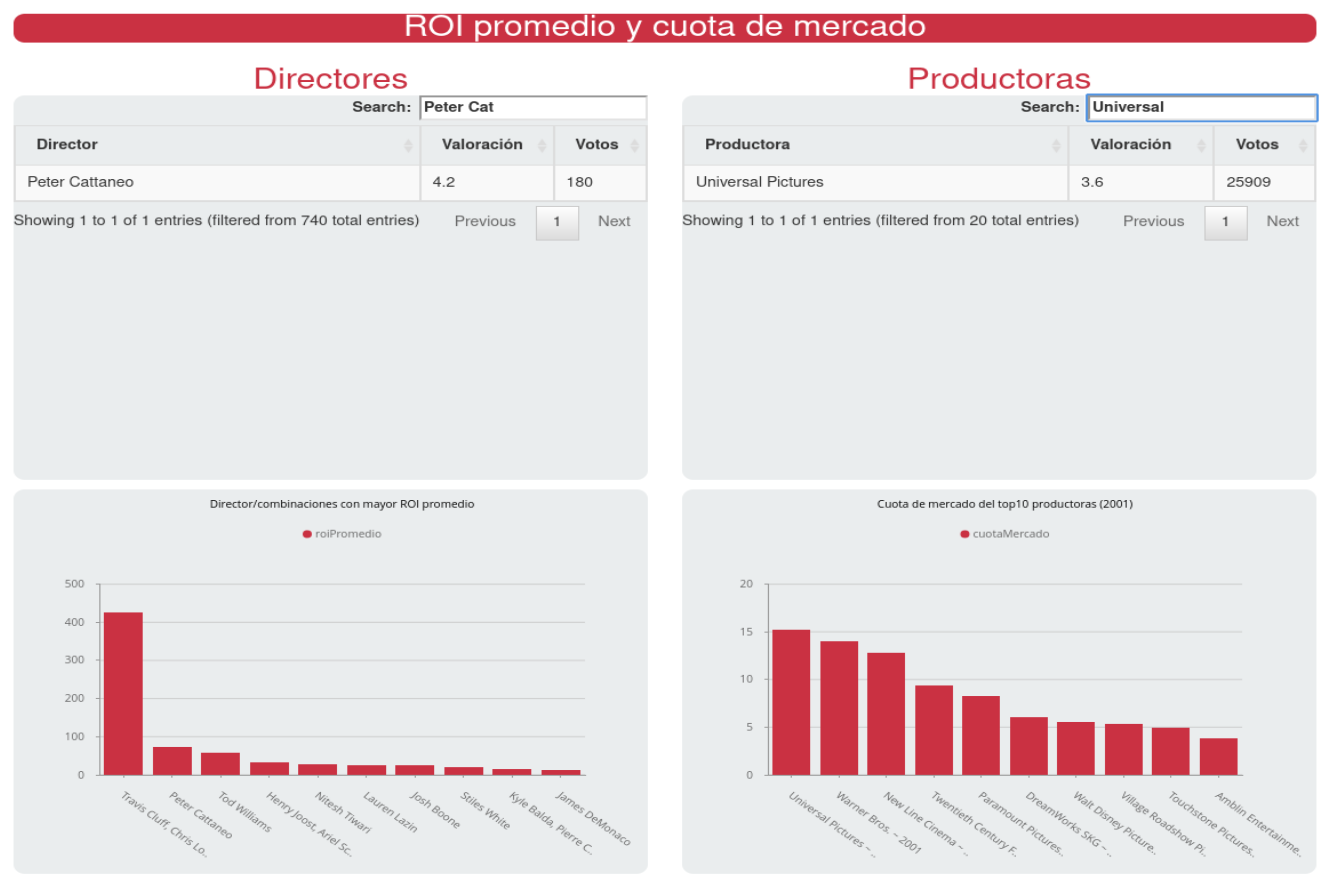
\includegraphics[width=0.7\textwidth]{fotos/1.png}
\caption{Representación de la flexibilidad vs interpretabilidad de distintos métodos.}
\label{fig:1}
\end{figure}

\subsection{Aprendizaje supervisado y no supervisado}

La gran mayoría de los problemas de aprendizaje estadístico entran un una de estas dos categorías: supervisado o no supervisado. Todo lo visto hasta ahora se trata de aprendizaje supervisado: para cada observación de un predictor $x_i$, $i = 1, \dots, n$, hay una salida asociada $y_i$. \\

Por el contrario, el aprendizaje no supervisado describe la situación en la que para cada observación se tiene un vector de medidas $x_i$, pero no una salida asociada $y_i$. En este contexto, se busca comprender las relaciones entre las variables o entre las observaciones. Un ejemplo en el \textit{clustering}.El objetivo de este método es establecer, en la base $x_1, \dots, x_n$, si una observación cae dentro de grupos relativamente distintos; se limita a buscar agrupaciones de datos que distingan un subconjunto de otro. Esto se puede ver en la figura \ref{fig:2}.

\begin{figure}[h]
\centering
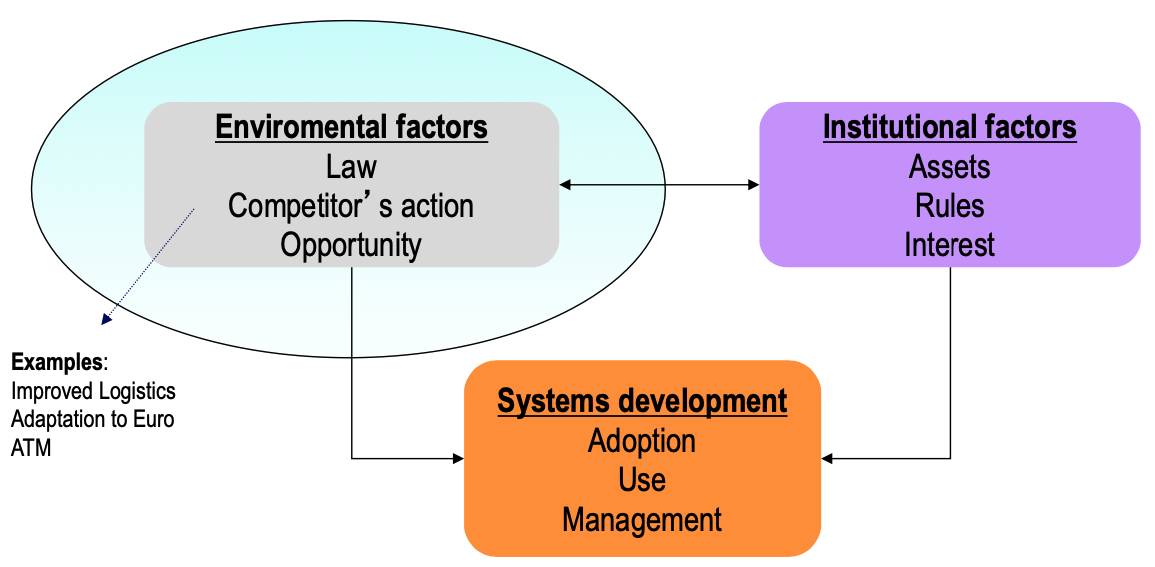
\includegraphics[width=0.7\textwidth]{fotos/2.png}
\caption{\textit{Clusters} de datos en un conjunto de observaciones. A la izquierda se observan tres grupos bien distinguidos, mientras que a la derecha la separación es más difusa.}
\label{fig:2}
\end{figure}

También existen metodos semisupervisados, donde se tiene la salida correspondiente a una fracción de las observaciones y no al total. En el caso de querer considerar las $n$ observaciones, tengan o no salida correspondiente, habría que usar este tipo de métodos. 

\subsection{Problemas de regresión y clasificación}

Las variables puedes caracterizarse como cuantitativas o cualitativas (categóricas). Generalmente, los problemas que involucran respuestas cuantitativas son de regresión, mientras que los que involucran respuestas cualitativas son de clasificación (sin atender a la naturaleza de los predictores). Sin embargo, algunos métodos estadísticos, como K-vecinos más próximos, pueden usarse para mabos tipos de variables. 